\chapter{Forward Model}
\label{ch:formodel}
In this chapter we present the forward model to which we apply all our methodology on. We follow the MIPAS handbook \cite{mipas2000handbook} and simulate data according to a cloud-free atmosphere in local thermodynamic equilibrium and assume a measurement instrument with infinite spectral resolution and no pointing errors.
\begin{figure}[ht!]
	\centering
	\input{LIMB.pdf_tex}
	\caption[Schematic of measurement and analysis geometry.]{Schematic of measurement and analysis geometry, not to scale.
		The stationary satellite, at a constant height $h_\text{sat}$ above Earth, takes $m = 41$ measurements along its line-of-sight defining by the line $\Gamma_j$.
		Each measurement has a limb height $\ell_j$, $j=1,2,\dots,m$ defined as the closest distance of $\Gamma_j$ to the Earth surface.
		Between $h_{L,0} = 7$km and $h_{L,n} = 83.3$km, the stratosphere is discretised into $n =44$ layers as illustrated by the solid green lines.}
	\label{fig:LIMB}
\end{figure}


A satellite at a constant height $h_{\text{sat}}$ points through the atmosphere (limb-sounding) and measures thermal radiation of gas molecules along its line of sight, see  Figure~\ref{fig:LIMB}.
One measurement of the thermal radiation if we target one specific molecule, in our case ozone denoted by the ozone volume mixing ratio $x(r)$ at distance $r$ from the satellite, of at the wave number $\nu$ is given by the path integral
\begin{align}
	\label{eq:RTE} 
	y_j =   \int_{\Gamma_j}  B(\nu,T) k(\nu, T)   \frac{p(T)}{k_{\text{B}} T(r)}  x(r)  \tau(r) \text{d}r + \eta_j \, \\
	\tau(r) = \exp{ \Bigl\{ - \int^{r}_{r_\text{obs}}  k(\nu, T)   \frac{p(T)}{k_B T(r^{\prime})}  x(r^{\prime}) \text{d}r^{\prime} \Bigr\} } \, ,\label{eq:absRTE} 
\end{align}
which is the radiative transfer equation (RTE)~\cite{mipas2000handbook} where we define a tangent height $h_{\ell_j}$ and a pointing direction is $\Gamma_j$ for each $j=1,2,\ldots,m$ measurement of the data vector $\bm{y} \in \mathbb{R}^m$ including some noise $\eta_j$.
Within the atmosphere the number density $p(T) / (k_{\text{B}} T(r))$ of molecules is dependent on the pressure $p(T)$, the temperature $T(r)$, and the Boltzmann constant $k_{\text{B}}$.
The factor $\tau(r)\leq 1$ accounts for re-absorption of the radiation along the line-of-sight, which makes the RTE non linear.
The absorption constant
\begin{align}
	k(\nu, T) = L(\nu, T_{\text{ref}}) \frac{Q(T_{\text{ref}})}{Q(T)} \frac{ \exp{\{ - c_2 E^{\prime \prime} / T\}} }{\exp{\{ - c_2 E^{\prime \prime} / T_{\text{ref}} \}}} \frac{ 1- \exp{\{ - c_2 \nu  / T \}} }{1 - \exp{\{ - c_2 \nu / T_{\text{ref}} \}}}
\end{align}
is depend on the line intensity $L(\nu, T_{\text{ref}})$ at reference temperature $T_{\text{ref}} =296K $, the lower-state energy of the transition $ E^{\prime \prime} $, the second radiation constant $c2=1.4387769\text{cmK}$ all provided by the HITRAN database \cite{gordon2022hitran2020}.
Since we assume that the measurement deceive as negligible frequency window we neglect line broadening around $\nu_0$ the calculations of $L(\nu, T_{\text{ref}})$ normally include broadening modelled as a convolution of the normalized Lorentz profile (collisional/pressure broadening) and the normalised Doppler (thermal broadening) profile \cite{}.
Additionally we note that we simplify the calculation of $k(\nu, T)$, which usually the sum the individual absorption constant for each targeted molecule weighted by the respective volume mixing ratio \cite{}.
Then the total internal partition function for the lower-state energy is
\begin{align}
	Q(T )= g^{\prime \prime} \exp{\{ - \frac{ c_2 E^{\prime \prime} }{T}\}} \, ,
\end{align}
with the statistical weight $ g^{\prime \prime}$ (also called the degeneracy factor) accounting for the molecules non-rotational and rotational energy states, see \cite{vsimevckova2006einstein}.
Under the assumption of local thermodynamic equilibrium (LTE) the black body radiation act as a source function
\begin{align}
	B(\nu,T)   = \frac{2 h c^2 \nu^3}{\exp{\{\frac{hc\nu}{k_B T}\}}-1}\, ,
\end{align}
with Planck's constant $h$ and velocity of light $c$ \cite{}.
For fundamentals on the Radiative transfer equation we recommend \cite[Chapter 1]{rybicki2000rte}.

To enable matrix-vector multiplication, we discretise the atmosphere in $n$ layers, where the $i^\text{th}$ layer is defined by two spheres of radii $h_{L,i-1} < h_{L,i}$, for $i = 1, \dots, n$, with $h_{L,0}$ and $h_{L,n} $.
Then we can discretise the ozone, pressure and temperature profiles as a function of height, where in between the heights $h_{L,i-1}$ and $h_{L,i}$, each of the ozone concentration $x_{i}$, the pressure $p_{i}$, the temperature $T_{i}$, as well as all other height dependent parameters are assumed to be constant.
Above $h_{L, n}$ and below $h_{L,0} $, the ozone concentration is set to zero, so no signal can be obtained.
Depending on the parameter of interest, which is either the ozone volume mixing ratio $\bm{x} =\{x_1,x_2,\ldots,x_n\} \in \mathbb{R}^{n}$ or the fraction of pressure and temperature $\bm{p/T}= \{p_1/T_1,p_2/T_2,\ldots,p_n/T_n\} \in \mathbb{R}^{n} $
we rewrite the integral in Eq.~\eqref{eq:RTE} for one noise free measurement using the trapezoidal rule as a vector-vector multiplication $\bm{A_{j}}(\bm{x},  \bm{p},\bm{T}) \, \bm{x} $ or $\bm{A_{j}}(\bm{x},  \bm{p},\bm{T}) \, \bm{p}/ \bm{T} $, where the non-linear absorption $\tau(r)$ is included in $\bm{A_{j}}(\bm{x},  \bm{p},\bm{T}) \in \mathbb{R}^{n}$ which is the $j$-th row of the matrix $\bm{A}(\bm{x},  \bm{p},\bm{T})$.
Then given a noise vector $\bm{\eta} \in \mathbb{R}^{m}$ the data vector
\begin{align}
	\bm{y} = \bm{A}_{NL} \, \bm{x} + \bm{\eta}= \bm{A}_{NL} \,
	\frac{ \bm{p}}{\bm{T}} + \bm{\eta} \, 
\end{align}
is based on a matrix-vector multiplication, where we define $\bm{A}(\bm{x},  \bm{p},\bm{T}) \equiv \bm{A}_{NL} \in \mathbb{R}^{m \times n}$ for simplicity so that $\bm{A}_{NL}\bm{x}$ or $\bm{A}_{NL}\bm{p}/\bm{T}$ implies the construction of $\bm{A}_{NL}$.
If we neglect the absorption, e.g. set $\tau = 1$ in Eq.~\eqref{eq:absRTE}, this problem becomes a linear problem with the forward model given by $\bm{A}_{L}\bm{x}$ or $\bm{A}_{L}\bm{p}/\bm{T}$. 
Further, we classify the inverse problem as weakly non-linear, see e.g. Fig. \ref{fig:MapAsses}, as neglecting the absorption changes the measurement only slightly.

\section{Singular value decomposition of linear forward model matrix}
In this section we want to give an intuitive way of how we can measure most effectively depending on the information passed through the forward model and how the signal to noise ratio affects that information.
One way of doing this is via a singular value decomposition (SVD) of the forward model matrix
\begin{align}
	\bm{A} = \sum_{i =1}^{r} \bm{u}_i  \sigma_i \bm{v}^T_i = \bm{U} \bm{\Sigma} \bm{V}^T
\end{align}
where $r = \min\{m,n\}$ for $\bm{A} \in \mathbb{R}^{m \times n}$.
One way of thinking about the SVD when considering a parameter $\bm{x}$, which is passed though the froward model as in $\bm{A}\bm{x}$, is that the right singular vectors $\bm{v}_i$ span the parameter space.
So if the right singular vectors are flat in heigh altitudes the forward model does not pick up any structure of the parameter in that region.
Then the right singular vectors are weighted with the singular values $\sigma_i$, which are ordered in size from the largest $\sigma_1$ to the smallest $\sigma_{r}$ singular value.
Lastly, the left singular vectors $ \bm{u}_i$ project to the data space.
See \cite{tan2016LecNot} for a more comprehensive analysis.

If we consider very small singular values below a threshold negligible we can introduce an effective rank $r_{\text{eff}} \leq r$, then $ \{\bm{v}_{r_{\text{eff}} +1}, \dots ,\bm{v}_r \}$ spans the null space, see Figure \ref{fig:nullSpac}.
This threshold may be affected by noise in the data.
If the rough assumption that the maximum singular value $\max(y) \approx \sigma_1$ holds and the signal-to-noise-ratio (SNR) is defined as 
\begin{align}
	\text{SNR} \coloneqq \frac{\max(y)}{\text{std. noise}}
\end{align}
then we can eye ball the information transmitted through the forward model, which are roughly the singular values $s_i \gtrsim \max(y)/ \text{SNR}$.

\begin{figure}[ht!]
	\centering
	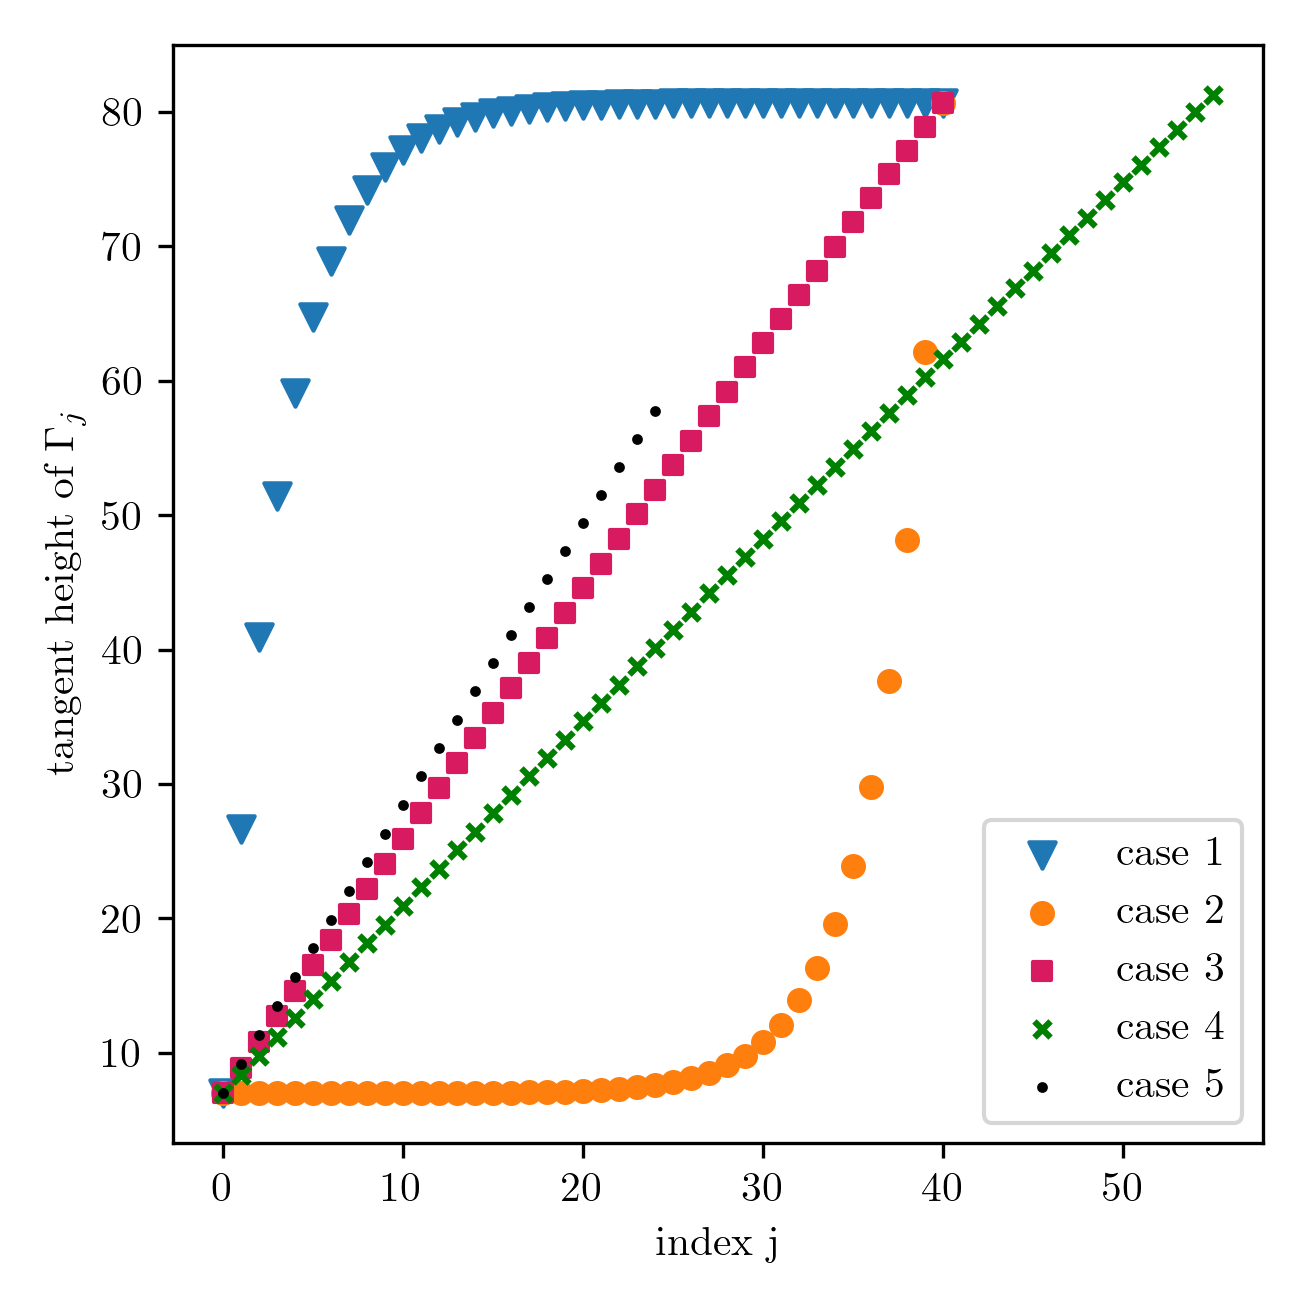
\includegraphics{MeasTangHeight.png}
	\caption[Tangent heights for different sequence of measurements.]{We plot the tangent heights for different cases of measurements.}
	\label{fig:TangHCases}
\end{figure}
\begin{figure}[ht!]
	\centering
	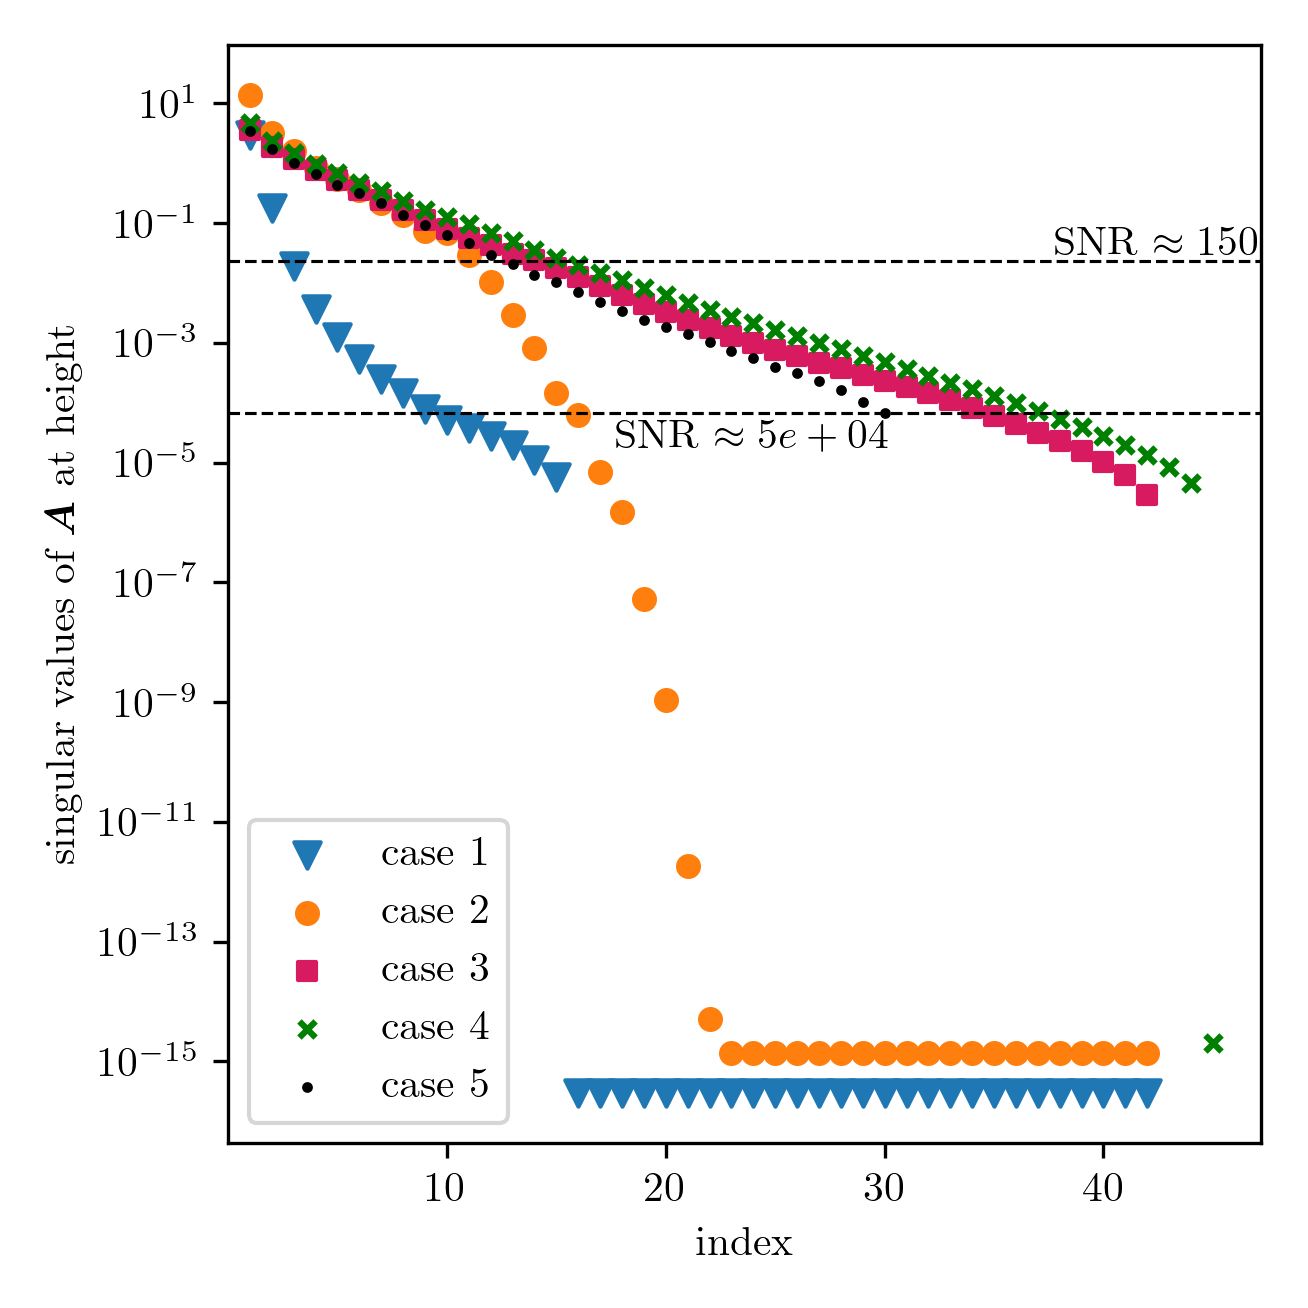
\includegraphics{SingValA.png}
	\caption[Singular values of linear forward model matrix for different sequences of measurements.]{We plot the singular values of linear forward model matrix for different sequences of measurements.
		The corresponding tangent heights of the different cases are plotted in Fig. \ref{fig:TangHCases}. We include an approximate for the disiered Signal to noise ratio if $s_1 \approx max(\bm{y}) $ the signal.}
	\label{fig:SingA}
\end{figure}
Next we analyse the singular values for a few different measurement scenarios, to see which of those measurement cases is most effective.
We test for different pointing accuracies, which determines how well the satellite can point in a certain direction, and we correlate that to the number of measurements.
The singular values for measurements with equally distanced tangent heights in between a set atmosphere, see case 3 in Fig. \ref{fig:TangHCases}, are plotted in Fig. \ref{fig:SingA}.
The pointing accuracy of $150\text{arc sec}$, was given to us by the team in \cite{CubeSatInternal}.
We can see that value of the singular values are linearly decreasing in log space (exponentially in normal space) and that we can roughly capture information of the first 15 to 20 singular values. 
In comparison, if we measure with exponentially decreasing pointing accuracy, see case 1 Fig. \ref{fig:TangHCases}, or increasing pointing accuracy, see case 2 Fig. \ref{fig:TangHCases}, the forward model does not give us more information.
We actually get fewer large singular values for case 2 and more very small singular values as we measure more in higher altitude where noise is dominant due to decreasing pressure and hence density.
Similarly case 2 does also not seem better than case 3, as we do get some larger singular values which then decease rapidly.
Also if we would half the pointing accuracy and double the number of measurements, case 4 in Fig. \ref{fig:TangHCases}, we do not increase the amount of information through our forward model.
Since I assume it is easier to build a satellite with lower pointing accuracy we find through exploratory analysis that we can tolerate a pointing accuracy of $150\text{arc sec}$ without much loss of information above a SNR of around 100.
And since we see that measuring more does not give more information we only measure until around 60 km in height, where the data start to get dominated by noise.
Consequently ozone values at higher altitudes are not determined by data but by the prior and given these singular values we can show quite clearly the ill-posedness of this model/problem.
Of course, if we increase the SNR by a factor of $10^5$ we would be able to see ozone peaks around 60km but that does not seem realistic.

\begin{figure}[ht!]
	\centering
	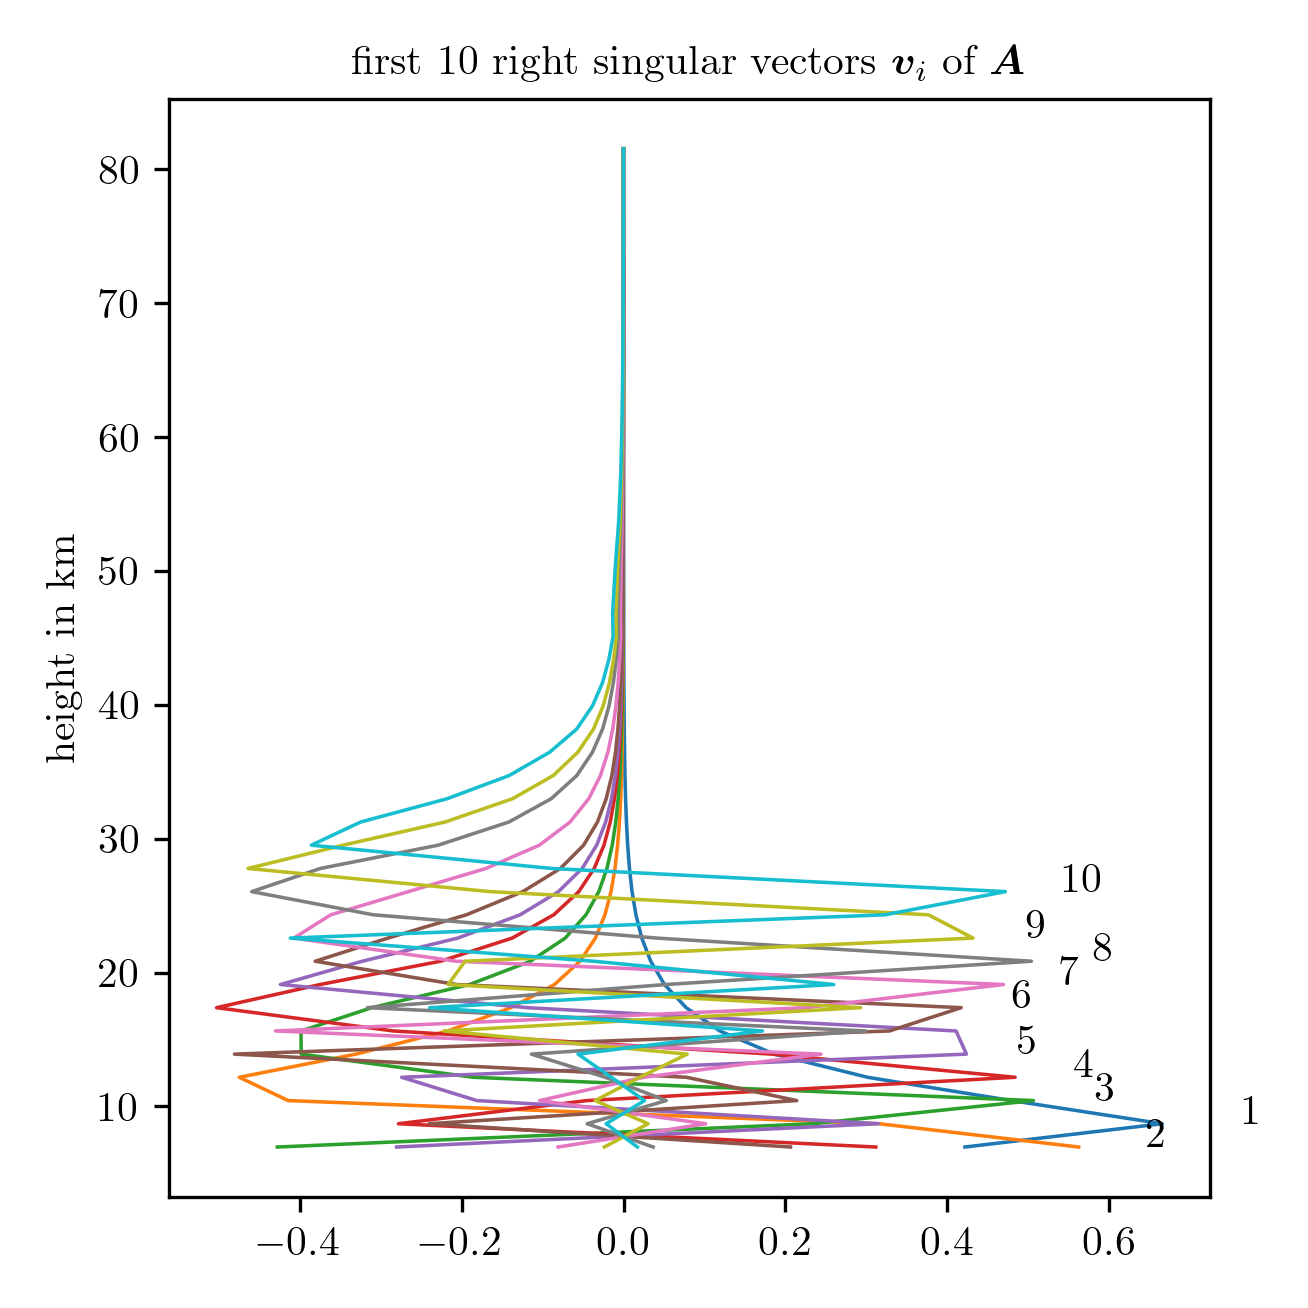
\includegraphics{SingVecA.png}
	\caption[Left singular vectors of forward model matrix for one sequence of measurements.]{We plot the first 20 left singular vectors of forward model matrix for case 5 sequence of measurements, see Fig. \ref{fig:SingA}.}
	\label{fig:SingVecA}
\end{figure}
\begin{figure}[ht!]
	\centering
	%\includegraphics{}
	\caption[]{}
	\label{fig:nullSpace}
\end{figure}
Consequently we proceed with case 5 and plot the parameter space of the model for the first 20 of 25 or so right singular vectors in Fig. \ref{fig:SingVecA}
We observe that we do not pick up structures above 60km.
The last 5 right singular vectors (null space) include structures above 60 km and hence our model is not sensitive to those.

\cite{livesey2006retrieval} Says that the instrument spents more time in lower regions, this does not increase perfomance !!!






%Hence, we can approximate the non-linear forward model $\bm{A}(\bm{x},  \bm{p},\bm{T})$ with a map $\bm{M}$ and the linear forward model $\bm{A}_L$, so that $\bm{A}(\bm{x},  \bm{p},\bm{T}) \approx \bm{M} \bm{A}_L $.
%Here, $\bm{A}_{L,j} $ of matrix $\bm{A}_L \in \mathbb{R}^{m \times n}$ is defined by the linear forward model, where absorption is neglected, e.g. set $\tau = 1$ in Eq.~\eqref{eq:absRTE}. 
%Then each entry in the row vector $\bm{A}_{L,j} $ is either defined by $ B(\nu) k(\nu)   \frac{\bm{p}}{k_{\text{B}} \bm{T}}  \text{d}r$ or $B(\nu) k(\nu)   \frac{\bm{x}}{k_{\text{B}}}  \text{d}r$, as in Eq.~\eqref{eq:RTE}.
%This poses a linear inverse problem with the forward map defined by the matrix $\bm{A} = \bm{M} \bm{A}_L$, where $\bm{M}$ is, more specifically, an affine map.


%\textcolor{red}{$h_{L,0}$ does not influences the values for $p_{L,O}/T_{L,0}$}
%\textcolor{red}{dont include bend of the line integral}

%\begin{figure}[ht!]
%	\centering
%	\scalebox{0.9}{\input{FirstLIMB.pdf_tex}}
%	\caption[General schematics of measurement setup]{This figure illustrates a limb-sounding measurement setup, specifically how the line of sight of a satellite at altitude $h_{\text{obs}}$ is partitioned according to a discretised atmospheric model. The atmosphere is divided into $n$ layers, allowing the line of sight $\Gamma_j$ to be discretised into segments $\Delta r_i$ for $i = \ell_j, \dots, n$.
%		Here, $\ell_j \in \mathbb{N}$ denotes the index corresponding to the tangent height $h_{\ell_j}$ relative to the Earth's radius $R_E$. This setup forms the basis for the numerical solution of the integral in Eq.~\ref{eq:RTE}, known as the radiative transfer equation.}
%	\label{fig:FirstLIMB}
%\end{figure}

%The absorption constant $k(\nu, T)$ for a single gas molecule at a specific wave number $\nu$ is calculated according to the HITRAN database \cite{gordon2022hitran2020} and acts as a source function when multiplied with the black body radiation $B(\nu,T)$, given by Planck`s law~\cite{rybicki2000rte}.
%We calculate the source function $B(\nu, T)$ and the absorption constant $ k(\nu, T)$ as follows.
%assumption local thermaodynamic equilibrium
%For one species at one specific wave-number the weighted absorption constant becomes
%\begin{align}
%	\overline{k(\nu, T, r)}    = \sum_{m=1}^{molec} k_m(\nu, T) x_m(r) =  k(\nu, T) x(r) \, ,
%\end{align}
%with the volume mixing ratio of ozone $x(r)$ at location $r$. 